% Options for packages loaded elsewhere
\PassOptionsToPackage{unicode}{hyperref}
\PassOptionsToPackage{hyphens}{url}
%
\documentclass[
]{article}
\usepackage{amsmath,amssymb}
\usepackage{lmodern}
\usepackage{iftex}
\ifPDFTeX
  \usepackage[T1]{fontenc}
  \usepackage[utf8]{inputenc}
  \usepackage{textcomp} % provide euro and other symbols
\else % if luatex or xetex
  \usepackage{unicode-math}
  \defaultfontfeatures{Scale=MatchLowercase}
  \defaultfontfeatures[\rmfamily]{Ligatures=TeX,Scale=1}
\fi
% Use upquote if available, for straight quotes in verbatim environments
\IfFileExists{upquote.sty}{\usepackage{upquote}}{}
\IfFileExists{microtype.sty}{% use microtype if available
  \usepackage[]{microtype}
  \UseMicrotypeSet[protrusion]{basicmath} % disable protrusion for tt fonts
}{}
\makeatletter
\@ifundefined{KOMAClassName}{% if non-KOMA class
  \IfFileExists{parskip.sty}{%
    \usepackage{parskip}
  }{% else
    \setlength{\parindent}{0pt}
    \setlength{\parskip}{6pt plus 2pt minus 1pt}}
}{% if KOMA class
  \KOMAoptions{parskip=half}}
\makeatother
\usepackage{xcolor}
\usepackage[margin=1in]{geometry}
\usepackage{color}
\usepackage{fancyvrb}
\newcommand{\VerbBar}{|}
\newcommand{\VERB}{\Verb[commandchars=\\\{\}]}
\DefineVerbatimEnvironment{Highlighting}{Verbatim}{commandchars=\\\{\}}
% Add ',fontsize=\small' for more characters per line
\usepackage{framed}
\definecolor{shadecolor}{RGB}{248,248,248}
\newenvironment{Shaded}{\begin{snugshade}}{\end{snugshade}}
\newcommand{\AlertTok}[1]{\textcolor[rgb]{0.94,0.16,0.16}{#1}}
\newcommand{\AnnotationTok}[1]{\textcolor[rgb]{0.56,0.35,0.01}{\textbf{\textit{#1}}}}
\newcommand{\AttributeTok}[1]{\textcolor[rgb]{0.77,0.63,0.00}{#1}}
\newcommand{\BaseNTok}[1]{\textcolor[rgb]{0.00,0.00,0.81}{#1}}
\newcommand{\BuiltInTok}[1]{#1}
\newcommand{\CharTok}[1]{\textcolor[rgb]{0.31,0.60,0.02}{#1}}
\newcommand{\CommentTok}[1]{\textcolor[rgb]{0.56,0.35,0.01}{\textit{#1}}}
\newcommand{\CommentVarTok}[1]{\textcolor[rgb]{0.56,0.35,0.01}{\textbf{\textit{#1}}}}
\newcommand{\ConstantTok}[1]{\textcolor[rgb]{0.00,0.00,0.00}{#1}}
\newcommand{\ControlFlowTok}[1]{\textcolor[rgb]{0.13,0.29,0.53}{\textbf{#1}}}
\newcommand{\DataTypeTok}[1]{\textcolor[rgb]{0.13,0.29,0.53}{#1}}
\newcommand{\DecValTok}[1]{\textcolor[rgb]{0.00,0.00,0.81}{#1}}
\newcommand{\DocumentationTok}[1]{\textcolor[rgb]{0.56,0.35,0.01}{\textbf{\textit{#1}}}}
\newcommand{\ErrorTok}[1]{\textcolor[rgb]{0.64,0.00,0.00}{\textbf{#1}}}
\newcommand{\ExtensionTok}[1]{#1}
\newcommand{\FloatTok}[1]{\textcolor[rgb]{0.00,0.00,0.81}{#1}}
\newcommand{\FunctionTok}[1]{\textcolor[rgb]{0.00,0.00,0.00}{#1}}
\newcommand{\ImportTok}[1]{#1}
\newcommand{\InformationTok}[1]{\textcolor[rgb]{0.56,0.35,0.01}{\textbf{\textit{#1}}}}
\newcommand{\KeywordTok}[1]{\textcolor[rgb]{0.13,0.29,0.53}{\textbf{#1}}}
\newcommand{\NormalTok}[1]{#1}
\newcommand{\OperatorTok}[1]{\textcolor[rgb]{0.81,0.36,0.00}{\textbf{#1}}}
\newcommand{\OtherTok}[1]{\textcolor[rgb]{0.56,0.35,0.01}{#1}}
\newcommand{\PreprocessorTok}[1]{\textcolor[rgb]{0.56,0.35,0.01}{\textit{#1}}}
\newcommand{\RegionMarkerTok}[1]{#1}
\newcommand{\SpecialCharTok}[1]{\textcolor[rgb]{0.00,0.00,0.00}{#1}}
\newcommand{\SpecialStringTok}[1]{\textcolor[rgb]{0.31,0.60,0.02}{#1}}
\newcommand{\StringTok}[1]{\textcolor[rgb]{0.31,0.60,0.02}{#1}}
\newcommand{\VariableTok}[1]{\textcolor[rgb]{0.00,0.00,0.00}{#1}}
\newcommand{\VerbatimStringTok}[1]{\textcolor[rgb]{0.31,0.60,0.02}{#1}}
\newcommand{\WarningTok}[1]{\textcolor[rgb]{0.56,0.35,0.01}{\textbf{\textit{#1}}}}
\usepackage{graphicx}
\makeatletter
\def\maxwidth{\ifdim\Gin@nat@width>\linewidth\linewidth\else\Gin@nat@width\fi}
\def\maxheight{\ifdim\Gin@nat@height>\textheight\textheight\else\Gin@nat@height\fi}
\makeatother
% Scale images if necessary, so that they will not overflow the page
% margins by default, and it is still possible to overwrite the defaults
% using explicit options in \includegraphics[width, height, ...]{}
\setkeys{Gin}{width=\maxwidth,height=\maxheight,keepaspectratio}
% Set default figure placement to htbp
\makeatletter
\def\fps@figure{htbp}
\makeatother
\setlength{\emergencystretch}{3em} % prevent overfull lines
\providecommand{\tightlist}{%
  \setlength{\itemsep}{0pt}\setlength{\parskip}{0pt}}
\setcounter{secnumdepth}{-\maxdimen} % remove section numbering
\ifLuaTeX
  \usepackage{selnolig}  % disable illegal ligatures
\fi
\IfFileExists{bookmark.sty}{\usepackage{bookmark}}{\usepackage{hyperref}}
\IfFileExists{xurl.sty}{\usepackage{xurl}}{} % add URL line breaks if available
\urlstyle{same} % disable monospaced font for URLs
\hypersetup{
  pdftitle={Tutorial on proteomics analysis using proteoDA},
  pdfauthor={Stephanie Byrum},
  hidelinks,
  pdfcreator={LaTeX via pandoc}}

\title{Tutorial on proteomics analysis using proteoDA}
\author{Stephanie Byrum}
\date{2023-01-20}

\begin{document}
\maketitle

\hypertarget{installation}{%
\subsection{Installation}\label{installation}}

\hypertarget{how-to-install-proteoda-from-github}{%
\subsubsection{How to install proteoDA from
Github:}\label{how-to-install-proteoda-from-github}}

\begin{enumerate}
\def\labelenumi{\arabic{enumi}.}
\tightlist
\item
  install devtools
\item
  install from github repo
\end{enumerate}

\begin{Shaded}
\begin{Highlighting}[]
\FunctionTok{install.packages}\NormalTok{(}\StringTok{"devtools"}\NormalTok{)}
\FunctionTok{library}\NormalTok{(devtools)}
\NormalTok{devtools}\SpecialCharTok{::}\FunctionTok{install\_github}\NormalTok{(ByrumLab}\SpecialCharTok{/}\NormalTok{proteoDA)}
\end{Highlighting}
\end{Shaded}

\hypertarget{data-import-and-requirements}{%
\subsection{Data Import and
Requirements}\label{data-import-and-requirements}}

ProteoDA utilizes an S3 object called DAList to hold the data and
results. DA stands for differential abundance and contains 7 slots
including: data, annotation, metadata, design, eBayes\_fit, results, and
tags. The first three slots are required.

data = a data frame or matrix containing protein intensity values for
each sample where the rows are proteins and the columns are samples. The
column sample names must match the row names of the metadata!

annotation = a data frame containing protein accession numbers,
description, gene symbols, etc. A column titled ``uniprot\_id'' is
required and case specific.

metatdata = a data frame containing sample information such as sample
name, group, gender, batch, etc. The rownames of the metadata must match
the column names of the data!

\begin{Shaded}
\begin{Highlighting}[]
\NormalTok{input }\OtherTok{\textless{}{-}} \FunctionTok{read.csv}\NormalTok{(}\StringTok{"vignette/DIA\_data.csv"}\NormalTok{)  }\CommentTok{\# subset the data and annotation}
\NormalTok{data }\OtherTok{\textless{}{-}}\NormalTok{ input[,}\DecValTok{5}\SpecialCharTok{:}\DecValTok{21}\NormalTok{]}
\NormalTok{anno }\OtherTok{\textless{}{-}}\NormalTok{ input[,}\DecValTok{1}\SpecialCharTok{:}\DecValTok{4}\NormalTok{]}
\NormalTok{meta }\OtherTok{\textless{}{-}} \FunctionTok{read.csv}\NormalTok{(}\StringTok{"vignette/metafile.csv"}\NormalTok{)}
\FunctionTok{row.names}\NormalTok{(meta) }\OtherTok{\textless{}{-}}\NormalTok{ meta}\SpecialCharTok{$}\NormalTok{data\_column\_name}

\CommentTok{\# create the proteoDA DAList object using the following command}

\NormalTok{DA }\OtherTok{\textless{}{-}} \FunctionTok{DAList}\NormalTok{(data,}
\NormalTok{            anno,}
\NormalTok{            meta,}
            \AttributeTok{design =} \ConstantTok{NULL}\NormalTok{,}
            \AttributeTok{eBayes\_fit =} \ConstantTok{NULL}\NormalTok{,}
            \AttributeTok{results =} \ConstantTok{NULL}\NormalTok{,}
            \AttributeTok{tags =} \ConstantTok{NULL}\NormalTok{)}

\end{Highlighting}
\end{Shaded}

\hypertarget{sample-and-protein-filtering-options}{%
\section{Sample and Protein filtering
options}\label{sample-and-protein-filtering-options}}

If a sample is detected as an outlier, it can be removed using the
filter\_samples() function and setting the condition parameter to
``sample\_name != sample-to-be-removed''. Samples are kept if the
condition is TRUE for that sample.

Proteins that contain missing values in the majority of samples can be
removed using the filter\_proteins\_by\_group() function. A general rule
of thumb is to require at least 2/3 of the replicates to have a value in
at least one sample group.

Example: If two groups have triplicate samples, then set min\_reps = 2
and min\_groups = 1. This removes proteins that do not have at least 2
out of 3 replicates in one sample group with an intensity value
\textgreater{} 0.

\begin{Shaded}
\begin{Highlighting}[]
\CommentTok{\# filter samples {-}{-}{-}{-}{-}{-}{-}{-}{-}{-}{-}{-}{-}{-}{-}{-}{-}{-}{-}{-}{-}{-}{-}{-}{-}{-}{-}{-}{-}{-}{-}{-}{-}{-}{-}{-}{-}{-}{-}{-}{-}{-}{-}{-}{-}{-}{-}{-}{-}{-}{-}{-}{-}{-}{-}{-}{-}{-}{-}{-}{-}{-}}
\NormalTok{sub\_data }\OtherTok{\textless{}{-}} \FunctionTok{filter\_samples}\NormalTok{(DA, group }\SpecialCharTok{!=} \StringTok{"Pool"}\NormalTok{)}

\CommentTok{\# filter proteins {-}{-}{-}{-}{-}{-}{-}{-}{-}{-}{-}{-}{-}{-}{-}{-}{-}{-}{-}{-}{-}{-}{-}{-}{-}{-}{-}{-}{-}{-}{-}{-}{-}{-}{-}{-}{-}{-}{-}{-}{-}{-}{-}{-}{-}{-}{-}{-}{-}{-}{-}{-}{-}{-}{-}{-}{-}}

\NormalTok{filtered\_data }\OtherTok{\textless{}{-}} \FunctionTok{filter\_proteins\_by\_group}\NormalTok{(sub\_data,}
                                          \AttributeTok{min\_reps =} \DecValTok{2}\NormalTok{,}
                                          \AttributeTok{min\_groups =} \DecValTok{1}\NormalTok{,}
                                          \AttributeTok{grouping\_column =} \StringTok{"group"}\NormalTok{)}
\end{Highlighting}
\end{Shaded}

\hypertarget{proteinorm-normalization}{%
\subsection{ProteiNorm Normalization}\label{proteinorm-normalization}}

proteiNorm is a tool developed to evaluate 8 popular normalization
methods: log2, mean, median, vsn, quantile, cyclic loess, robust linear
regression (rlr), and global intensity normalization (gi). Each method
is evaluated using pooled coefficient of variance, pooled estimate
variance, pooled median absolute deviation, intragroup correlation, and
log2 ratios. More information can be found at
\url{https://github.com/ByrumLab/proteiNorm}.

proteiNorm is now available as a part of proteoDA workflow. After
evaluating the proteiNorm.pdf report, the best normalization method can
be selected using the normalize\_data() function.

References: Graw S, Tang J, Zafar MK, Byrd AK, Bolden C, Peterson EC,
Byrum SD. proteiNorm - A User-Friendly Tool for Normalization and
Analysis of TMT and Label-Free Protein Quantification. ACS Omega. 2020
Sep 30;5(40):25625-25633. doi: 10.1021/acsomega.0c02564. PMID: 33073088;
PMCID: PMC7557219.

Normalyzer: A Tool for Rapid Evaluation of Normalization Methods for
Omics Data Sets Aakash Chawade, Erik Alexandersson, and Fredrik Levander
Journal of Proteome Research 2014 13 (6), 3114-3120 DOI:
10.1021/pr401264n

\begin{Shaded}
\begin{Highlighting}[]
\CommentTok{\# Normalization report {-}{-}{-}{-}{-}{-}{-}{-}{-}{-}{-}{-}{-}{-}{-}{-}{-}{-}{-}{-}{-}{-}{-}{-}{-}{-}{-}{-}{-}{-}{-}{-}{-}{-}{-}{-}{-}{-}{-}{-}{-}{-}{-}{-}{-}{-}{-}{-}{-}{-}{-}{-}}

\FunctionTok{write\_norm\_report}\NormalTok{(filtered\_data,}
                  \AttributeTok{grouping\_column =} \StringTok{"group"}\NormalTok{,}
                  \AttributeTok{output\_dir =} \StringTok{"01\_QC\_report"}\NormalTok{,}
                  \AttributeTok{filename =} \StringTok{"proteiNorm.pdf"}\NormalTok{,}
                  \AttributeTok{overwrite =}\NormalTok{ T,}
                  \AttributeTok{suppress\_zoom\_legend =} \ConstantTok{FALSE}\NormalTok{,}
                  \AttributeTok{use\_ggrastr =} \ConstantTok{FALSE}\NormalTok{)}

\NormalTok{norm }\OtherTok{\textless{}{-}} \FunctionTok{normalize\_data}\NormalTok{(filtered\_data,}
                       \AttributeTok{norm\_method =} \StringTok{"cycloess"}\NormalTok{)}
\end{Highlighting}
\end{Shaded}

\hypertarget{proteinorm_report.pdf-results}{%
\subsection{ProteiNorm\_report.pdf
Results}\label{proteinorm_report.pdf-results}}

\#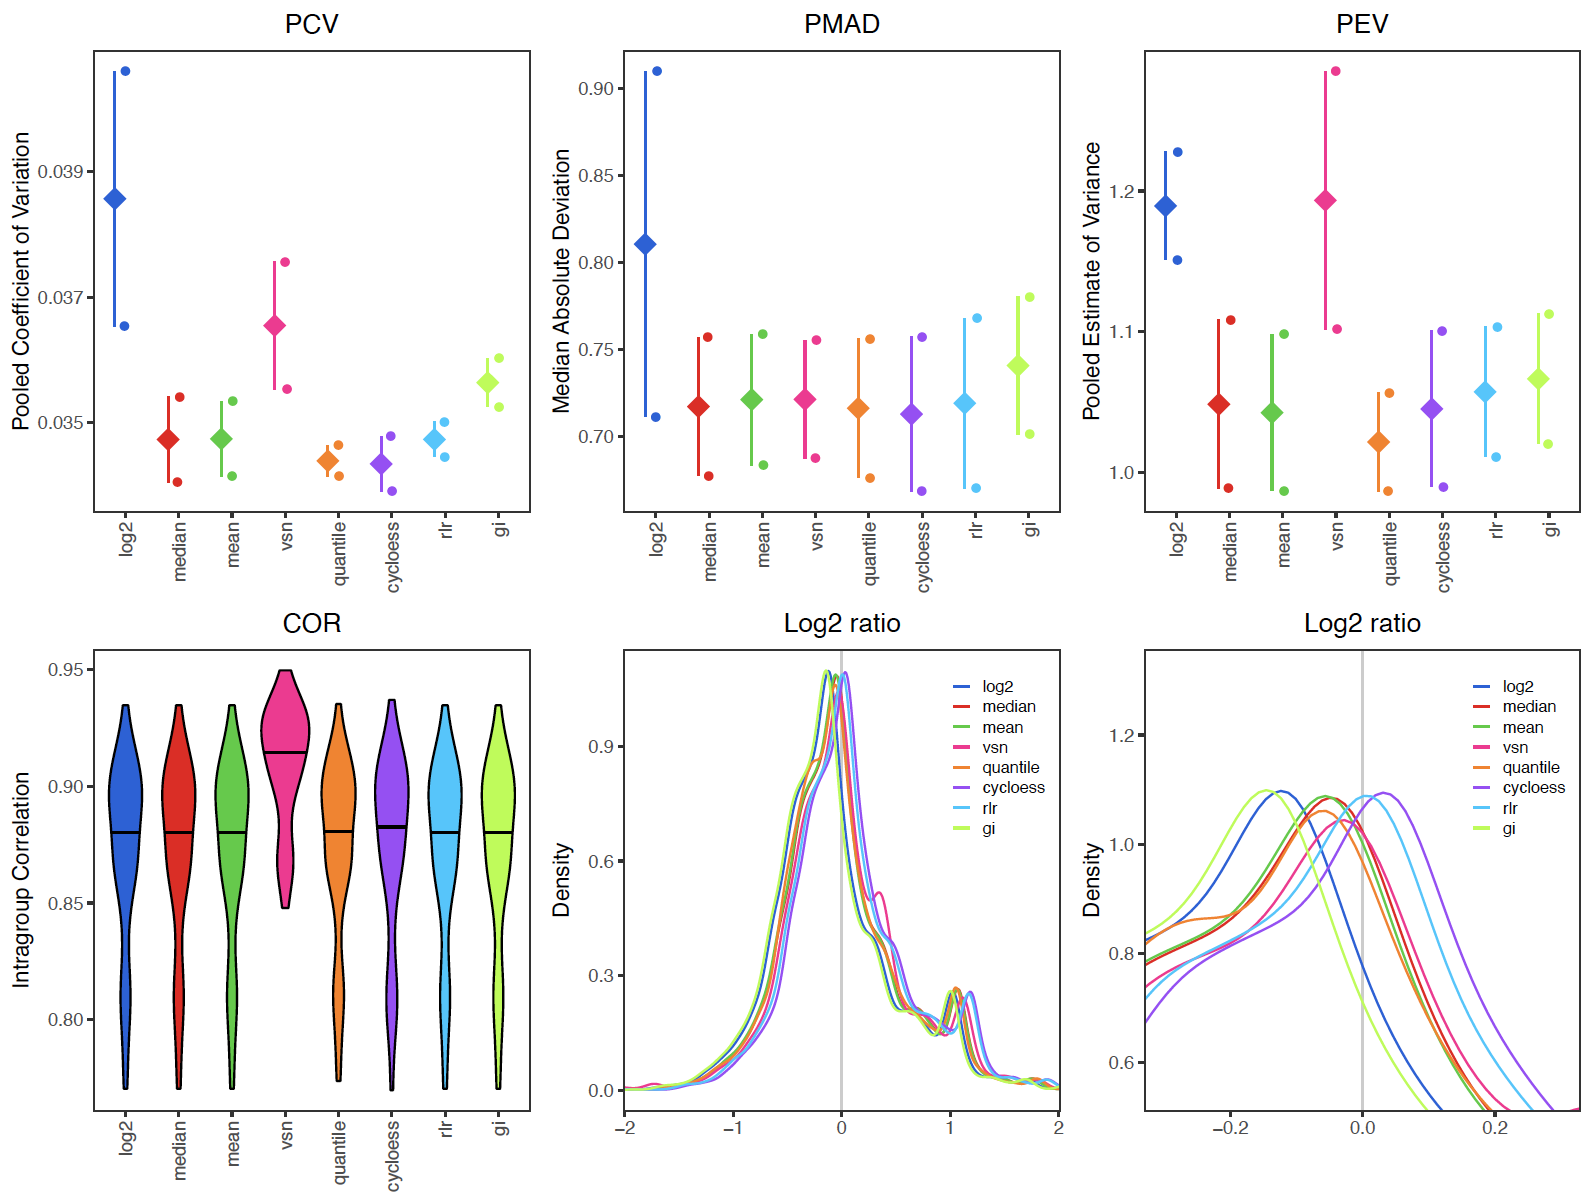
\includegraphics{https://github.com/sbyrum21/proteoDA/blob/tutorial/images/proteiNorm.png}

\hypertarget{quality-control-report}{%
\subsection{Quality Control Report}\label{quality-control-report}}

Once the normalization method has been chosen, QC plots are generated
using the selected normalized data. The QC report generates violin
plots, PCA, clustered dendrograms, correlation heatmap of each sample,
and a plot of proteins with missing values.

Missing values in mass spectrometry do not mean the protein is not
present in the sample but rather the protein was not detected. This
might be due to the dynamic range limitations.

\begin{Shaded}
\begin{Highlighting}[]
\FunctionTok{write\_qc\_report}\NormalTok{(norm,}
                \AttributeTok{color\_column =} \StringTok{"group"}\NormalTok{,}
                \AttributeTok{label\_column =} \ConstantTok{NULL}\NormalTok{,        }\CommentTok{\# defaults to the metafile rownames}
                \AttributeTok{output\_dir =} \StringTok{"01\_QC\_report"}\NormalTok{,}
                \AttributeTok{filename =} \StringTok{"QC\_report.pdf"}\NormalTok{,}
                \AttributeTok{overwrite =}\NormalTok{ T,}
                \AttributeTok{top\_proteins =} \DecValTok{500}\NormalTok{,         }\CommentTok{\# number of most variable proteins for clustering}
                \AttributeTok{standardize =} \ConstantTok{TRUE}\NormalTok{,}
                \AttributeTok{pca\_axes =} \FunctionTok{c}\NormalTok{(}\DecValTok{1}\NormalTok{,}\DecValTok{2}\NormalTok{),          }\CommentTok{\# first 2 PCs}
                \AttributeTok{dist\_metric =} \StringTok{"euclidean"}\NormalTok{,  }\CommentTok{\# stats::dist for options}
                \AttributeTok{clust\_method =} \StringTok{"complete"}\NormalTok{,  }\CommentTok{\# stats::hclust for options}
                \AttributeTok{show\_all\_proteins =}\NormalTok{ F)  }\CommentTok{\# only those with missing data}
\end{Highlighting}
\end{Shaded}

\hypertarget{prepare-limma-model-design-and-sample-group-comparisons}{%
\subsection{Prepare limma model design and sample group
comparisons}\label{prepare-limma-model-design-and-sample-group-comparisons}}

The limma design formula must be added to the DAList() in order to run
the statistical analysis. A design matrix is a model matrix of
explanatory variables of a set of objects. Each row represents
individual samples and the columns represent the sample groups and
factors (such as batch).

The design formula is a string for the design matrix which can include
intercept (``\textasciitilde group''), no intercept (``\textasciitilde0
+ group''), additive (``\textasciitilde group + batch''), or interaction
(``\textasciitilde group*treatment) models.

If the no intercept model is selected, then the add\_contrasts()
function allows the user to provide the sample comparisons as a file or
a vector. This option allows for all pair-wise comparisons.

If the intercept model is selected, then the sample groups are compared
against the reference.

An excellent guide for design matrices is in the following reference.\\
Reference: Law CW, Zeglinski K, Dong X et al.~A guide to creating design
matrices for gene expression experiments {[}version 1; peer review: 2
approved{]}. F1000Research 2020, 9:1444
(\url{https://doi.org/10.12688/f1000research.27893.1})

\begin{Shaded}
\begin{Highlighting}[]
\NormalTok{norm }\OtherTok{\textless{}{-}} \FunctionTok{add\_design}\NormalTok{(norm,}
                   \AttributeTok{design\_formula =} \StringTok{"\textasciitilde{} 0 + group"}\NormalTok{)}


\NormalTok{norm }\OtherTok{\textless{}{-}} \FunctionTok{add\_contrasts}\NormalTok{(norm,}
                      \AttributeTok{contrasts\_file =} \StringTok{"vignette/contrasts.csv"}\NormalTok{)}
\end{Highlighting}
\end{Shaded}

\hypertarget{fit-the-limma-differential-abundance-model}{%
\subsection{Fit the limma differential abundance
model}\label{fit-the-limma-differential-abundance-model}}

Fits the limma differential abundance model to the intensity data,
following the specified design and (optional) contrast matrices. When a
random factor is included, uses limma::duplicateCorrelation to estimate
the intra-block correlation within groups.

Uses limma::lmFit to fit the initial model, optionally re-parameterizes
the results in terms of contrasts with limma::contrasts.fit, and then
recomputes moderated statistics following limma's empirical Bayes model
with limma::eBayes.

\begin{Shaded}
\begin{Highlighting}[]
\NormalTok{fit }\OtherTok{\textless{}{-}} \FunctionTok{fit\_limma\_model}\NormalTok{(norm)}

\CommentTok{\# Extract results {-}{-}{-}{-}{-}{-}{-}{-}{-}{-}{-}{-}{-}{-}{-}{-}{-}{-}{-}{-}{-}{-}{-}{-}{-}{-}{-}{-}{-}{-}{-}{-}{-}{-}{-}{-}{-}{-}{-}{-}{-}{-}{-}{-}{-}{-}{-}{-}{-}{-}{-}{-}{-}{-}{-}{-}{-}}
\NormalTok{results }\OtherTok{\textless{}{-}} \FunctionTok{extract\_DA\_results}\NormalTok{(fit,}
                              \AttributeTok{pval\_thresh =} \FloatTok{0.055}\NormalTok{,}
                              \AttributeTok{lfc\_thresh =} \DecValTok{1}\NormalTok{,}
                              \AttributeTok{adj\_method =} \StringTok{"BH"}\NormalTok{,}
                              \AttributeTok{extract\_intercept =}\NormalTok{ F)}

\CommentTok{\# Write results {-}{-}{-}{-}{-}{-}{-}{-}{-}{-}{-}{-}{-}{-}{-}{-}{-}{-}{-}{-}{-}{-}{-}{-}{-}{-}{-}{-}{-}{-}{-}{-}{-}{-}{-}{-}{-}{-}{-}{-}{-}{-}{-}{-}{-}{-}{-}{-}{-}{-}{-}{-}{-}{-}{-}{-}{-}{-}{-}}
\FunctionTok{write\_limma\_tables}\NormalTok{(results,}
                   \AttributeTok{output\_dir =} \StringTok{"02\_DA\_results"}\NormalTok{,}
                   \AttributeTok{overwrite =}\NormalTok{ T,}
                   \AttributeTok{contrasts\_subdir =} \ConstantTok{NULL}\NormalTok{,}
                   \AttributeTok{summary\_csv=}\ConstantTok{NULL}\NormalTok{,}
                   \AttributeTok{combined\_file\_csv =} \ConstantTok{NULL}\NormalTok{,}
                   \AttributeTok{spreadsheet\_xlsx =} \ConstantTok{NULL}\NormalTok{,}
                   \AttributeTok{add\_filter =}\NormalTok{ T)}

\FunctionTok{write\_limma\_plots}\NormalTok{(results,}
                  \AttributeTok{grouping\_column =} \StringTok{"group"}\NormalTok{,}
                  \AttributeTok{table\_columns =} \FunctionTok{c}\NormalTok{(}\StringTok{"uniprot\_id"}\NormalTok{,}\StringTok{"Protein.0me"}\NormalTok{),}
                  \AttributeTok{title\_column =} \StringTok{"uniprot\_id"}\NormalTok{,}
                  \AttributeTok{output\_dir =} \StringTok{"02\_DA\_results"}\NormalTok{,}
                  \AttributeTok{tmp\_subdir =} \StringTok{"tmp"}\NormalTok{,}
                  \AttributeTok{height =} \DecValTok{1000}\NormalTok{,}
                  \AttributeTok{width =} \DecValTok{1000}\NormalTok{)}

\end{Highlighting}
\end{Shaded}


\end{document}
